\section{\textsc {Task \uppercase\expandafter{\romannumeral3}}: Target Oriented Forest Management Strategy}

\subsection{Overview}
Forest management strategies outline the managers' or landowners' target for their forests, describe the status quo of the forests, and give a plan of actions to accomplish management targets \cite{plan}. To help forest managers or landowners make proper and efficient forest management, according to the EEC model, we divide forest development directions into three categories: ecological orientation ,economic orientation and cultural orientation, which correspond to the three development stages of the forest ecosystem: elementary, intermediate and advanced.


%To distinguish strategies above, we use Analytic Hierarchy Process (AHP) to determine the weights of each indicator, and embed these weights as impact factors into the EEC model to help forest managers determine the optimal harvesting volume and forest plan. All ratings are from experts and comparison matrices are checked for consistency.


%\begin{figure}[H]
%\centering
%\setlength{\abovecaptionskip}{0.cm}
%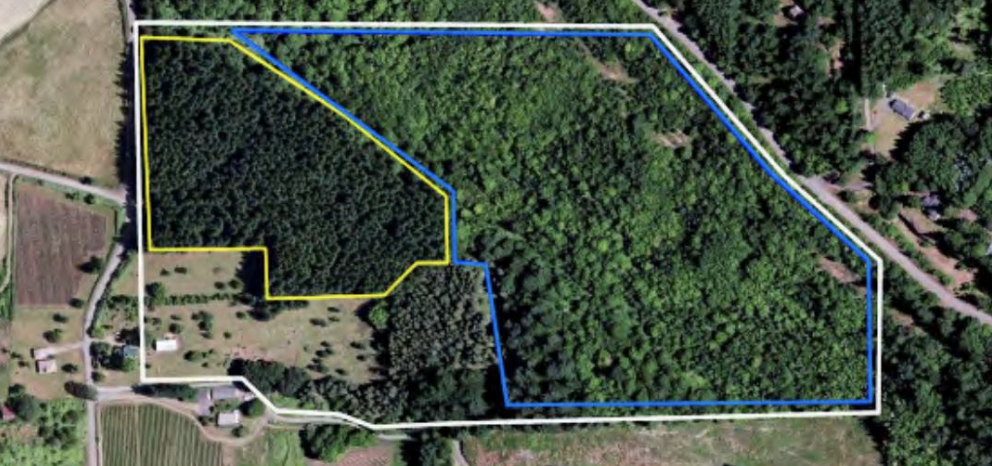
\includegraphics[scale = 0.75]{mcmthesis-demo/figures/plan.png}
%\caption{A forest management strategy, in which the yellow area is the growing area, the blue area is the mature area, and the rest part is used for other avenues (such as tourism, research and education, etc.)} 
%\end{figure}


%\begin{comment}The decision-making problem can be divided into three levels. The top level is the target layer M which selects the most appropriate method to evaluate the forest value and make the best forest management plan; The lowest layer is the scheme layer P including different quantitative indicators of forest value in EEC model. The middle layer is the criterion layer including three target forest management strategies: economic oriented strategy(C1), ecological oriented strategy(C2) and cultural oriented strategy(C3).


%The first step is to construct a judgment matrix. Different strategy orientations will use different criteria to construct judgment matrix, and compare the importance of evaluation methods in the criterion layer.\end{comment}

\subsection{Stage and Strategy}

\subsubsection{Elementary Stage: Ecologically Orientated Strategy}

This kind of forest management strategy is suitable for forests with sparse vegetation or damaged forests, which are vulnerable and poorly self-regulated. In this stage, managers or landowners should put the target of forest ecological protection in the first place by intervening in the forest to help forests restore growth quickly. Alternative decisions are listed below.

\begin{itemize}
\item \textbf{Protect soil and water}. Soil and water are vital to maintain the healthy operation of the forest ecosystem. For instance, managers can substitute native plants for invasive canary grass along the creek, which is harmful to water quality.
\item \textbf{Enhance wildlife habitat}. Species richness is an essential measure of forest health that we cannot ignore. Managers can improve the habitat for birds and other wildlife in the forest.
\item \textbf{Plant trees and afforest}. As the most significant contributor to carbon sequestration, trees play an indispensable role in the healthy functioning of forests, and planting trees properly will improve forest carbon sequestration.
\end{itemize}

\subsubsection{Intermediate Stage: Economically Orientated Strategy}

The intermediate stage is transitional in forest management. With the accumulation of forests' ecological value, we can turn the main target from ecological value to economic value. Specifically, the production and trade of forest products. In this process, the area's harvesting volume and product structure are the key factors. When the ecological value reaches a certain value, managers or landowners can change the development direction in time.

\begin{itemize}
\item \textbf{Conduct forest thinning regularly}. According to the SHG model, it is reasonable to say that for a healthy forest system, harvesting must be incorporated into the forest management plan to realize its comprehensive value. The optimal deforestation rate will be given by the SHG model.
\item \textbf{Adjust product structure}. Forest products are the main source of forest economic value. Different forest products have different profits. Managers can properly adjust the product structure to obtain greater benefits.
\end{itemize}
\subsubsection{Advanced Stage: Culturally Orientated Strategy}

This is the most advanced stage of forest management. At this stage, the forest has not only a rich ecological value and a stable economic value, but also the ability to create a cultural value. The most important source of a forest's cultural value is tourism and scientific research activities. Low-level forests are either unable to regulate themselves or lack sufficient economic support to carry too many tourists, and naturally cannot develop their cultural value. This is where culture-oriented forest management is advanced.

\begin{itemize}
\item \textbf{Develop tourism}. For high-level forests, the appropriate opening of tourism policies can improve the local spiritual and cultural level, and profit-making tourist attractions can also gain benefits and achieve a win-win situation.
\item \textbf{Establish research bases}. 
Due to the complex community structures and biological species, advanced forests have great potential research value.
\end{itemize}

\subsection{Implement of Forest Management Strategies by Decision Tree}
In decision analysis, a decision tree can be used to visually and explicitly represent decisions and decision making. As the name goes, it uses a tree-like model of decisions \cite{decision tree}. As one of machine learning algorithms, it takes features and targets as input, trains through a certain algorithm and builds a branched tree to make classification.

\subsubsection{Data Distribution}
In this section, we use the ecological, economic and cultural values percentage of different forests as features and three development stages of forests as targets for training. We selected 2,214 forests \cite{data of forest}, according to the ECC model, calculating the percentage of their ecological, economic and cultural values as feature input. Distribution of data is shown in Fig. [\ref{Data distribution in different dimensions}].

\begin{figure}[H]
\centering
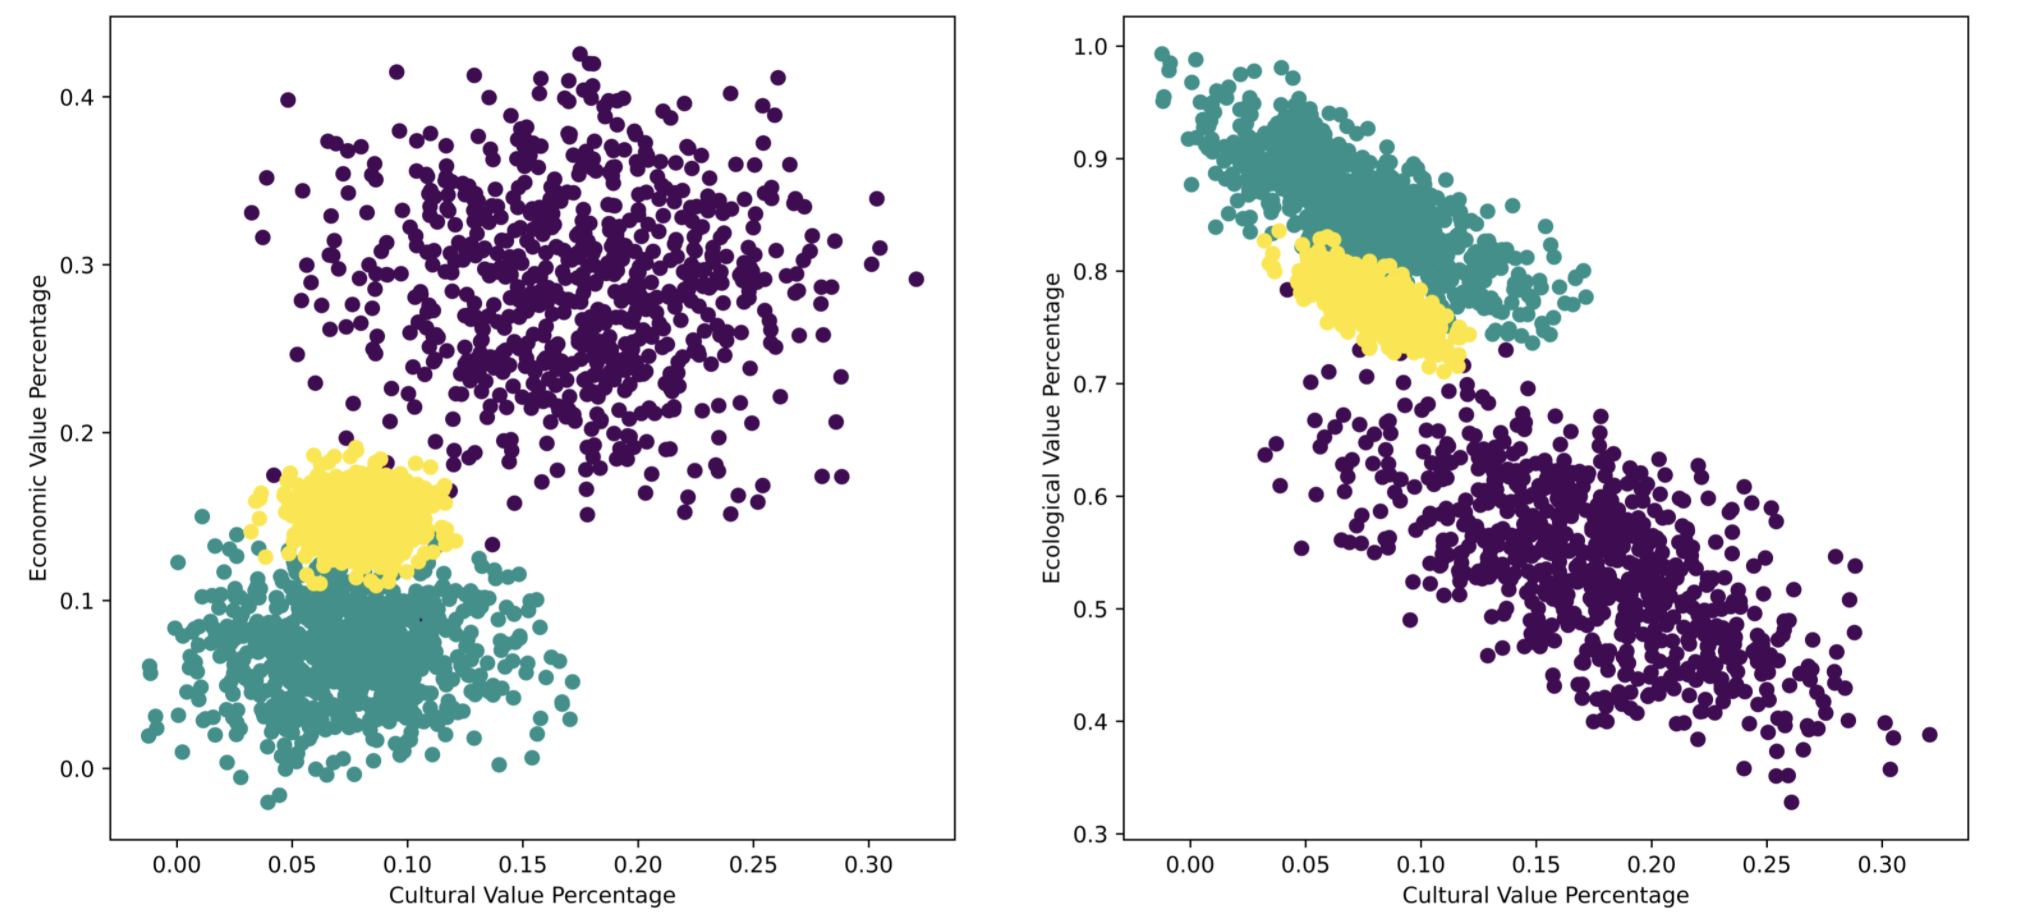
\includegraphics[scale = 0.4]{mcmthesis-demo/figures/Data.png}
\caption{Data distribution in different dimensions} 
\label{Data distribution in different dimensions}
\end{figure}

\subsubsection{Adjust the Parameters}
Among the total data, the training set accounts for 70\% of the total data, and the rest is used for testing. By decision tree algorithm, we can obtain the ideal classification plan of forest stage. Here, we set the count of random state as $i$ and depth of the decision tree as $j$.  By loop iteration of $i$ and $j$, we finally determine the most suitable random state as 190 and the max depth of the decision tree as 2. Then we choose the cross-validation method to test our model. The final accuracy reaches 96.54\%. The process of finding random state and max depth are shown in the following figures.

\begin{figure}[H]
\centering
\vspace{-1ex}
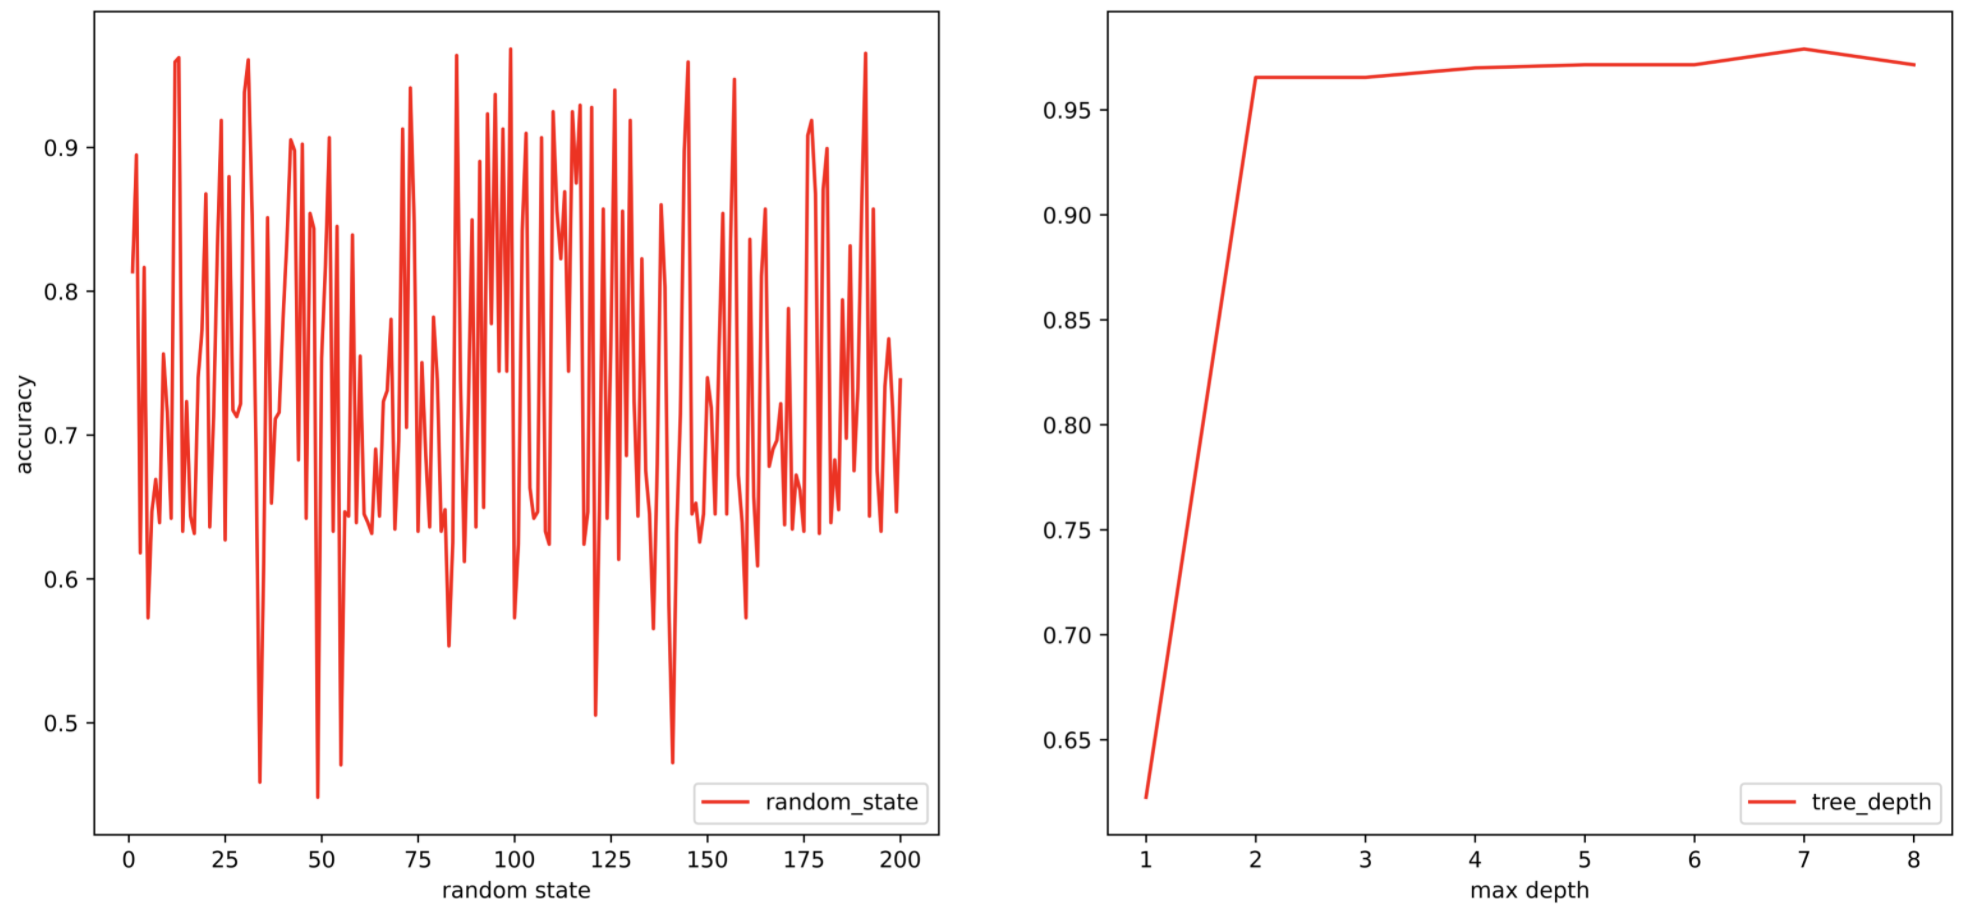
\includegraphics[scale = 0.4]{mcmthesis-demo/figures/Random State and Max Depth.png}
\vspace{-2ex}
\caption{Process of finding the best random state and tree depth} 
\end{figure}

\subsubsection{Strategies and Threshold Analysis}
Finally,we can draw the following decisions from our decision tree:

\begin{itemize}
    \item When the economic value ratio is greater than \textbf{10.8\%} and the ecological value is less than or equal to \textbf{69.5\%}, the forest is in the \textbf{primary stage}, where an \textbf{ecological-oriented} management strategy should be adopted.
    
    \item When the economic value ratio is greater than \textbf{10.8\%} and the ecological value is greater than \textbf{69.5\%}, the forest is at an \textbf{advanced stage}, and the development direction should be adjusted to a \textbf{culture-oriented} strategy.
    
    \item In other cases, the forest is at an \textbf{intermediate stage} and an \textbf{economic-oriented} management strategy should be adopted.
\end{itemize}

\begin{figure}[H]
\centering
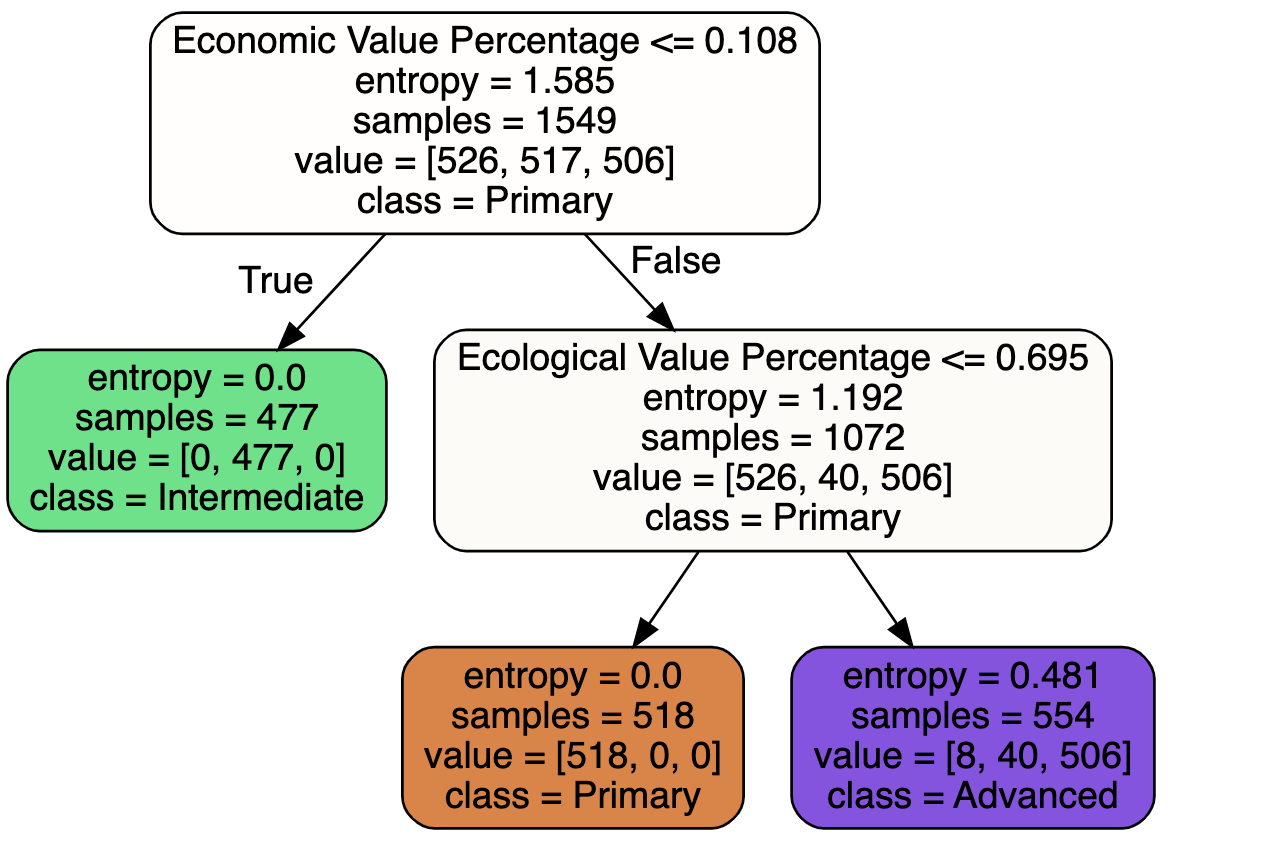
\includegraphics[scale = 0.45]{mcmthesis-demo/figures/Decision Tree Graph.png}
\caption{Decision tree graph} 
\end{figure}

Target Oriented Forest Management Strategy is the right handle for forest managers or landowners. They just need the forest parameter table for one year, use the SHG and ECC models to calculate the composition of the total valu. Then, by referring to the strategies, they can easily determine the stage of the forest and the future direction of development. The transition management plan appear near 10.8\% of economic value, which reminds forest managers and landowners not to harvest too much. Keeping the economic value near 10\% may be the best option.
